\documentclass{beamer}
\usepackage{amsmath, amsthm, amssymb}
\usepackage{color}
%\setbeamertemplate{items}[ball] 
\usepackage{aecompl,accents}
\usepackage[all]{xy}
\usepackage[normalem]{ulem}
\usepackage{mathtools}

\usepackage{graphicx}
\usepackage{hyperref}
%\usepackage[cache=false]{minted}

% Za pisanje psevdokode
\usepackage{algpseudocode}  % za psevdokodo
\usepackage{algorithm}
\floatname{algorithm}{Algoritem}
\renewcommand{\listalgorithmname}{Kazalo algoritmov}
\algnewcommand\algorithmicto{\textbf{to}}
\algnewcommand\algorithmicin{\textbf{in}}
\algnewcommand\algorithmicforeach{\textbf{for each}}
\algrenewtext{For}[3]{\algorithmicfor\ #1 $\gets$ #2\ \algorithmicto\ #3\ \algorithmicdo}
\algdef{S}[FOR]{ForEach}[2]{\algorithmicforeach\ #1\ \algorithmicin\ #2\ \algorithmicdo}
\newcommand{\algorithmicbreak}{\textbf{break}}
\newcommand{\Break}{\State \algorithmicbreak}


\usepackage{tikz}
\usetikzlibrary{math, overlay-beamer-styles}

%%%%%%%%%%%%%%%%%%%%%%%%%%%%%%%%%%%%%%%%%%%%%%%%%%%%%%%%%%%%
\usetheme{Ilmenau}
\usecolortheme{beaver}
\setbeamercolor{block title}{bg=darkred,fg=structure.fg!20!bg!50!bg}
\setbeamercolor{block body}{bg=black!2!red!4!white}
\setbeamercolor{local structure}{fg=darkred}
\setbeamercolor{item projected}{bg=darkred}
\setbeamercolor{titlelike}{parent=structure,bg=red!2!black!5!white}
\setbeamertemplate{title page}[default][rounded=false,shadow=false5]
\setbeamertemplate{enumerate items}[default]
\useinnertheme{rectangles}
\setbeamertemplate{blocks}[default]
\setbeamertemplate{navigation symbols}{}
\usefonttheme[onlymath]{serif}
\usepackage[slovene]{babel}
\usepackage[OT2,T1]{fontenc}
\usepackage[utf8]{inputenc}
%%%%%%%%%%%%%%%%%%%%%%%%%%%%%%%%%%%%%%%%%%%%%%%%%%%%%%%%%%%%%%%%%%%%%%%%%
\newtheorem{trditev}[theorem]{Trditev}
\newtheorem{izrek}[theorem]{Izrek}
\newtheorem{posledica}[theorem]{Posledica}
\newtheorem{definicija}{Definicija}
\newtheorem{domneva}[theorem]{Domneva}
%%%%%%%%%%%%%%%%%%%%%%%%%%%%%
\title[Ničelna prisila]{Ničelna prisila}
\author{Ines Meršak}
\date[25.9.2019]{Mentor: prof.~dr.~Sandi Klavžar}
%%%%%%%%%%%%%%%%%%%%%%%%%%%%%%%%%%%%%%%%%%%%%%%%%%%%%%%%%%%%%%%%%%%%%%%%%%
\newcommand{\N}{\ensuremath{\mathbb{N}}}
\newcommand{\R}{\ensuremath{\mathbb{R}}}
\newcommand{\F}{\ensuremath{\mathbb{F}}}
\DeclareMathOperator{\rang}{rang}
\DeclareMathOperator{\korang}{korang}
\DeclareMathOperator{\mr}{mr}
\DeclareMathOperator{\M}{M}
\DeclareMathOperator{\supp}{supp}
\newcommand{\squarep}{\mathbin{\square}}
\newcommand{\NP}{\ensuremath{\mathsf{NP}}}


\begin{document}

\frame{\titlepage}

\section{Uvod}
\begin{frame}[fragile,label=definicija]{Definicija}
    $ G = (V,E)$ končen enostaven neusmerjen graf

    \medskip
    
    \begin{enumerate}
        \item $Z \subset V$ množica črnih vozlišč, $V \setminus Z$ množica belih vozlišč
        \item $\forall u \in Z$, ki ima natanko enega belega soseda $v$, vozlišče $v$ pobarvamo črno
        \item drugo točko ponavljamo, dokler še lahko naredimo kakšno spremembo
    \end{enumerate}
    \begin{definicija}
        \alert{Množica ničelne prisile} je tak $Z \subset V$, da so po koncu zgornjega postopka vsa vozlišča $G$ pobarvana črno.
        $\alert{Z(G)} = \min \{|Z|\colon Z \subset V ,\ Z\text{ je množica ničelne prisile }G \} $
    \end{definicija}
\end{frame}

\begin{frame}{Primer}
    \begin{figure}
        \centering
        \begin{tikzpicture}
        \begin{scope}[every node/.style={circle,thick,draw}]
        \node[fill=black, fill on=<5->] (1) at (0,0) {};
        \node[fill=black, fill on=<2->] (2) at (0,2) {};
        \node[fill=black, fill on=<4->] (3) at (2,0) {};
        \node[fill=black, fill on=<3->] (4) at (2,2) {};
        \node[fill=black, fill on=<2->] (5) at (4,2) {};
        \end{scope}
        
        \path[-,thick,draw]
        (1) edge (2)
        (2) edge (3)
        (1) edge (3)
        (3) edge (4)
        (4) edge (5);
        \end{tikzpicture}
    \end{figure}
\end{frame}

\againframe{definicija}

\begin{frame}{Zgornja in spodnja meja}
    Za ničelno prisilo velja: 
    \[ Z(G) \leq n(G) - 1 \]
    \[ Z(G)  \geq 1 \]
    
    Spodnjo mejo lahko s krajšim premislekom hitro izboljšamo:
    \[ Z(G) \geq \delta(G) \]
\end{frame}

\begin{frame}{Motivacija}
    $S_n(\R)$ -- simetrične matrike $n\times n$
    
    \medskip
    
    $A \in S_n(\R) \colon$
    $\mathcal{G}(A)$ je graf z $n$ vozlišči in povezavami $\{\{i,j\}\colon a_{ij} \neq 0,\, 1 \leq i < j \leq n \} $
    
    \medskip
    \begin{definicija}
        $\mathcal{S}(G) = \{ A \in S_n(\R)\colon \mathcal{G}(A) = G \} $ \\
        $\mr(G) = \min \{ \rang A \colon A \in \mathcal{S}(G) \}$ \alert{minimalni rang} grafa $G$
        $M(G) = \max \{ \korang A \colon A \in \mathcal{S}(G) \}$ \alert{maksimalni korang} grafa $G$
    \end{definicija}
    
    \[ \mr(G) + M(G) = n(G) \]
\end{frame}

\begin{frame}{Primer}
    \begin{columns}
        \begin{column}{0.49\textwidth}
            \[ A = \begin{bmatrix*}[r]
            5 & -2 & 3 & 0 & 0 \\
            -2 & 13 & 6.9 & 0 & 0 \\
            3 & 6.9 & 0 & 7 & 0 \\
            0 & 0 & 7 & -1.1 & 1 \\
            0 & 0 & 0 & 1 & 0 \\
            \end{bmatrix*}\]
        \end{column}
        
        \begin{column}{0.5\textwidth}
            \begin{figure}
                \centering
                \begin{tikzpicture}
                \begin{scope}[every node/.style={circle,thick,draw}]
                \node (1) at (0,0) {1};
                \node (2) at (0,2) {2};
                \node (3) at (2,0) {3};
                \node (4) at (2,2) {4};
                \node (5) at (4,2) {5};
                \end{scope}
                
                \path[-,thick,draw]
                (1) edge (2)
                (2) edge (3)
                (1) edge (3)
                (3) edge (4)
                (4) edge (5);
                \end{tikzpicture}
            \end{figure}
        \end{column}
    \end{columns}
\end{frame}

\begin{frame}
    \begin{block}{Problem minimalnega ranga grafa}
        Določiti želimo parameter $\mr(G)$ za nek graf $G$.
    \end{block}
    
    \begin{trditev}
        $Z \subseteq V$ množica ničelne prisile grafa $G$. \\ 
        Velja $M(G) \leq |Z|$ in torej $M(G) \leq Z(G)$.
    \end{trditev}

    \begin{izrek}
        Za naslednje družine grafov velja $Z(G) = M(G)$:
        \begin{enumerate}
            \item vsi grafi $G$ z $|G| \leq 6$
            \item $P_n, C_n, K_n$
            \item drevesa
        \end{enumerate}
    \end{izrek}
\end{frame}


\section{Rezultati za nekatere razrede grafov}

\begin{frame}{Pot}
    \[ Z(P_n) = 1 \]
    \begin{figure}
        \centering
        \begin{tikzpicture}[scale=1.2]
        \begin{scope}[every node/.style={circle,thick,draw}]
        \foreach \i in {1,...,5}
        {
                \node[fill=black, fill on=<\i->] (\i) at (\i,0) {}; 
        }
        \end{scope}
        
        \foreach \i in {2,...,5}
        {
            \tikzmath{\im = int(\i-1);}
            \path[-,thick,draw] (\im) edge (\i); 
        }
                
        \end{tikzpicture}
    \end{figure}
    
    \[ Z(P_n) \geq \delta(P_n) = 1 \]
\end{frame}

\begin{frame}{Polni graf}
    \[ Z(K_n) = n-1 \]
    \begin{figure}
        \centering
        \begin{tikzpicture}[scale=0.7]
        \tikzmath{\n = 5; \r = 2.5; \nm = int(\n-1);}
        \begin{scope}[every node/.style={circle,thick,draw}]
        \foreach \i in {1,...,\n}
        {
            \ifthenelse{\i<2} {
                \node[fill=black, fill on=<2>] (\i) at ({90 + (360/\n * (\i - 1))}: \r) {}; } {
                \node[fill=black] (\i) at ({90 + (360/\n * (\i - 1))}: \r) {}; }
        }
        \end{scope}
        
        \foreach \i in {1,...,\nm}
        {
            \tikzmath{\ip = int(\i + 1);}
            \foreach \j in {\ip,...,\n} {
                \path[-,thick,draw] (\i) edge (\j); 
            }
        }
        \end{tikzpicture}
    \end{figure}
    
    \[ Z(K_n) \geq \delta(K_n) = n-1 \]
\end{frame}

\begin{frame}{Karakterizacija grafov z ekstremnimi $Z(G)$}
    \begin{trditev}
        \[ Z(G) = 1 \iff G = P_n \text{ za } n \geq 1 \]
    \end{trditev}
    
    \bigskip
    
    \begin{trditev}
        Naj bo $G$ povezan graf z $n(G) \geq 2$. Potem velja
        \[ Z(G) = n(G)-1 \iff G = K_{n(G)} \]
    \end{trditev}
\end{frame}

\begin{frame}{Cikel}
    \[ Z(C_n) = 2 \]
    
    \begin{figure}
        \centering
        \begin{tikzpicture}[scale=0.7]
        \tikzmath{\n = 7; \r = 2.5;}
        \begin{scope}[every node/.style={circle,thick,draw}]
        \foreach \i in {1,...,\n}
        {
            \tikzmath{\im = int(\i - 1);}
            \ifthenelse{\i>2} {
                \node[fill=black, fill on=<\im->] (\i) at ({360/\n * (\i - 1)}: \r) {}; } {
                \node[fill=black] (\i) at ({360/\n * (\i - 1)}: \r) {}; }
        }
        \end{scope}
        
        \foreach \i in {1,...,\n}
        {
            \tikzmath{\im = int(mod(\i,\n)+1);}
            \path[-,thick,draw] (\im) edge (\i);
        }
        \end{tikzpicture}
    \end{figure}
    
    \[ Z(C_n) \geq \delta(C_n) = 2 \]
\end{frame}

\begin{frame}{Zvezda}
    \[ Z(S_n) = n - 1\]
    \begin{figure}
        \centering
        \begin{tikzpicture}[scale=0.6]
            \tikzmath{\n = 6; \r = 2.5; \nm = int(\n-1);}
            \begin{scope}[every node/.style={circle,thick,draw}]
            \foreach \i in {1,...,\n} {
                \ifthenelse{\i<2} {
                    \node[fill=black, fill on=<3>] (\i) at ({90 + (360/\n * (\i - 1))}: \r) {}; } {
                    \node[fill=black] (\i) at ({90 + (360/\n * (\i - 1))}: \r) {}; }
            }
            \node[fill=black, fill on=<2->] (0) at (0,0) {};
            \end{scope}
            
            \foreach \i in {1,...,\n} {
                \path[-,thick,draw] (\i) edge (0); 
            }
        \end{tikzpicture}
    \end{figure}
\end{frame}

\begin{frame}{Kolo}
    \[ Z(W_n) = 3 \]
    \begin{figure}
        \centering
        \begin{tikzpicture}[scale=0.7]
        \tikzmath{\n = 7; \r = 2.5; \nm = int(\n-1);}
        \begin{scope}[every node/.style={circle,thick,draw}]
        \foreach \i in {1,...,\n} {
         \tikzmath{\imm = int(mod(\n + \i - 2, \n));}
         \ifthenelse{\i<2 \OR \i>4 } {
             \node[fill=black, fill on=<\imm->] (\i) at ({90 + (360/\n * (\i - 1))}: \r) {}; } {
             \node[fill=black] (\i) at ({90 + (360/\n * (\i - 1))}: \r) {}; }
        }
        \node[fill=black, fill on=<2->] (0) at (0,0) {};
        \end{scope}
        
        \foreach \i in {1,...,\n} {
            \tikzmath{\im = int(mod(\i,\n)+1);}
            \path[-,thick,draw] (\i) edge (0); 
            \path[-,thick,draw] (\i) edge (\im); 
        }
        \end{tikzpicture}
    \end{figure}
    
    \[ Z(W_n) \geq \delta(W_n) = 3 \]
\end{frame}

\section{Izračun}
\begin{frame}{Preverljivost}
    Ali obstaja množica ničelne prisile $\leq k$?
    
    \bigskip
    
    Želimo algoritem, ki preveri, ali je dana množica za dan graf res množica ničelne prisile.
    
    \bigskip
    
    Tri implementacije:
    \begin{itemize}
        \item naivna,
        \item z vrsto in množicami belih sosedov,
        \item z vrsto in seznamom števcev belih sosedov.
    \end{itemize}
\end{frame}

\begin{frame}{}
    Model Erdős–Rényi: vsako povezavo izberemo z verjetnostjo $p$. 
    \begin{figure}
        \centering
        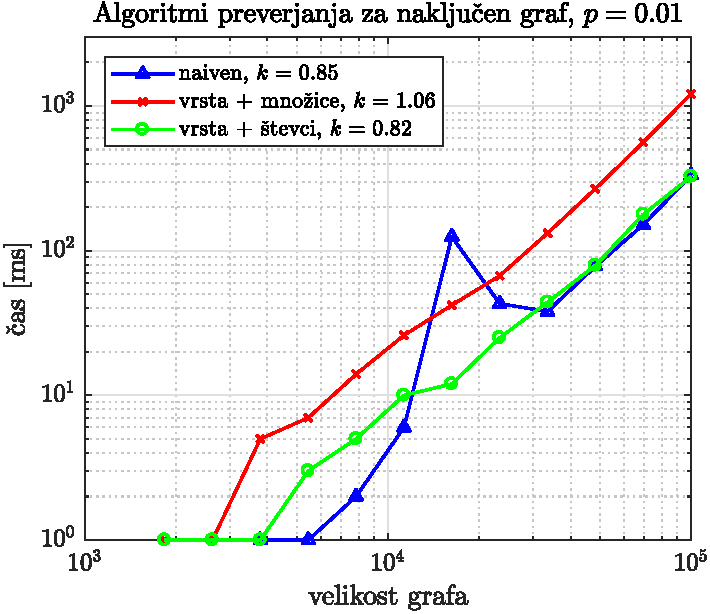
\includegraphics[width=0.49\linewidth]{../koda/results/plots/random_sparse.pdf}
        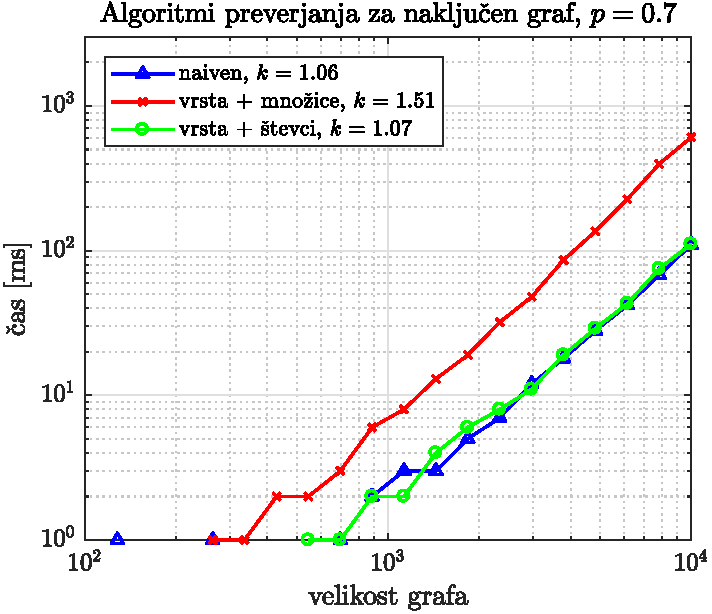
\includegraphics[width=0.49\linewidth]{../koda/results/plots/random_dense.pdf}
        \caption{Primerjava časov izvajanja v odvisnosti od velikosti grafa za naključno generirane grafe $G$ po modelu Erdős–Rényi.}
    \end{figure}
\end{frame}

\begin{frame}{}
    \begin{figure}
        \centering
        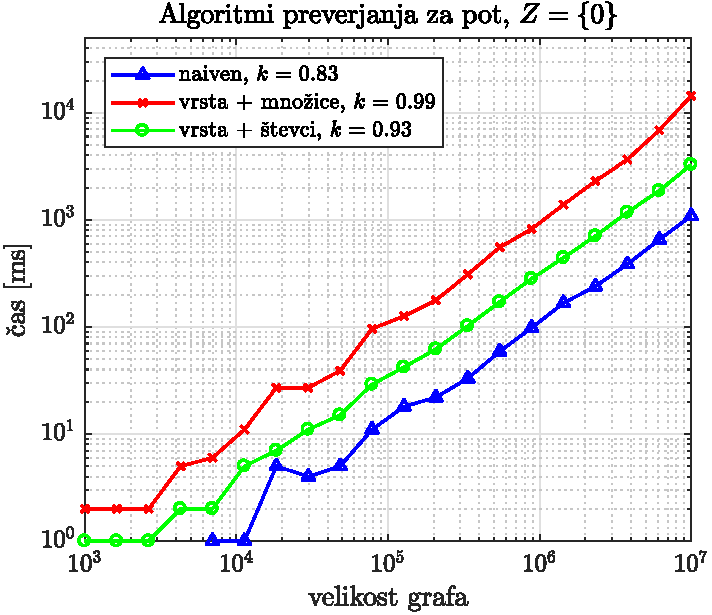
\includegraphics[width=0.49\linewidth]{../koda/results/plots/pot_prvo_vozlisce.pdf}
        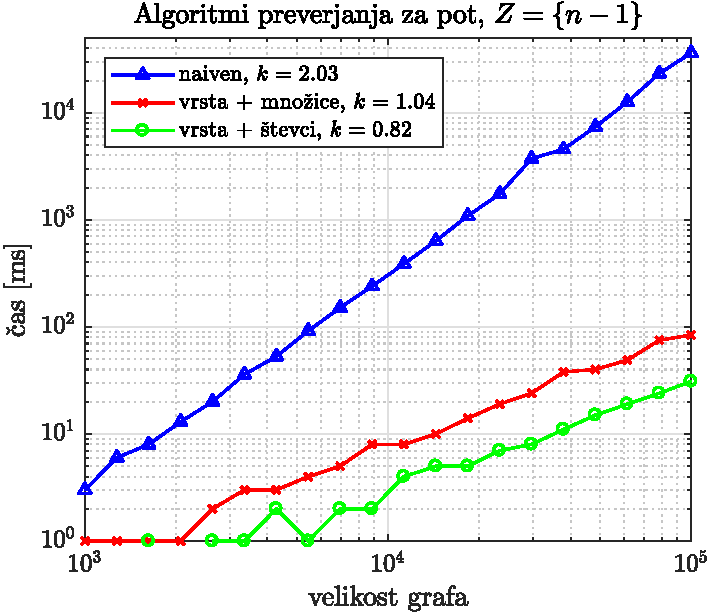
\includegraphics[width=0.49\linewidth]{../koda/results/plots/pot_zadnje_vozlisce.pdf}
        \caption{Primerjava časov izvajanja za poti v odvisnosti od velikosti; pri tem je na levi strani izbrana začetna množica $\{ 0 \}$, na desni pa $\{n-1\}$.}
    \end{figure}
\end{frame}

\begin{frame}{Eksponentni algoritem}
    \begin{algorithm}[H]
        \caption{}
        \raggedright
        \textbf{Vhod:} Graf $G = (V,E)$. \\
        \textbf{Izhod:} Število ničelne prisile $Z(G)$, $1 \leq Z(G) \leq n-1$.
        \begin{algorithmic}[1]
            \State $z \gets n+1$
            \ForEach{$Z$}{$2^V$}
            \If{$\Call{preveri}{G, Z} \land |Z| < z$}
            \State $z \gets |Z|$
            \EndIf
            \EndFor
            \State \Return $z$
        \end{algorithmic}
    \end{algorithm}
\end{frame}

\begin{frame}{}
    \begin{figure}
        \centering
        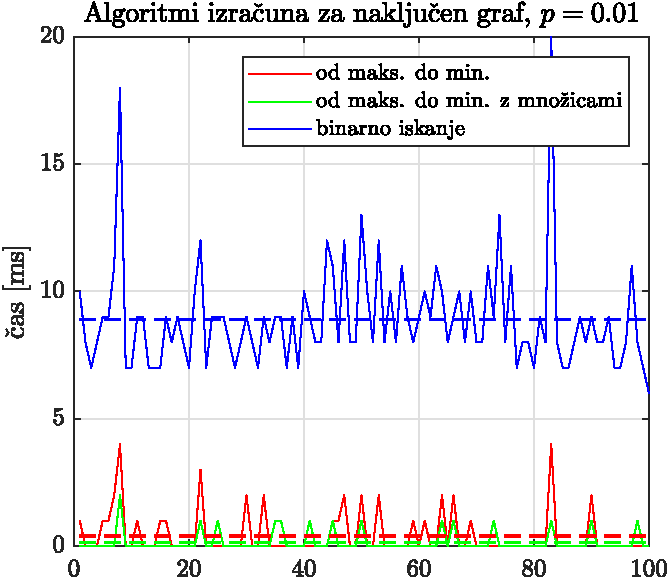
\includegraphics[width=120pt]{../koda/results/plots/zfn_random_15_sparse.pdf}
        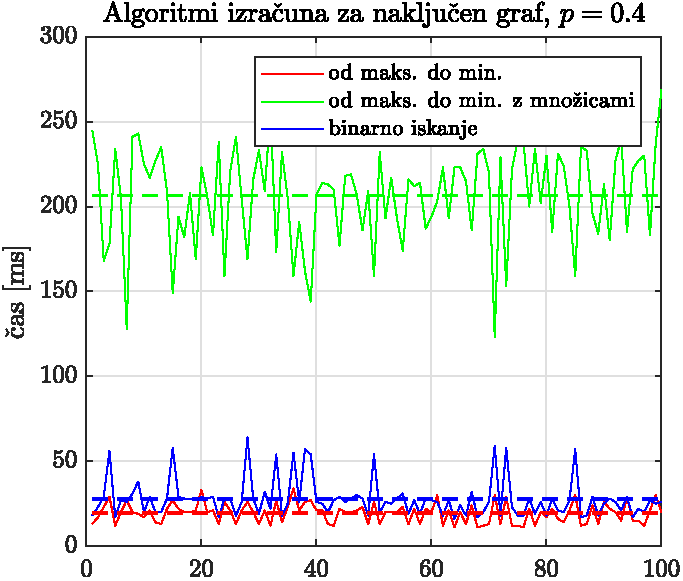
\includegraphics[width=120pt]{../koda/results/plots/zfn_random_15_mid.pdf}
        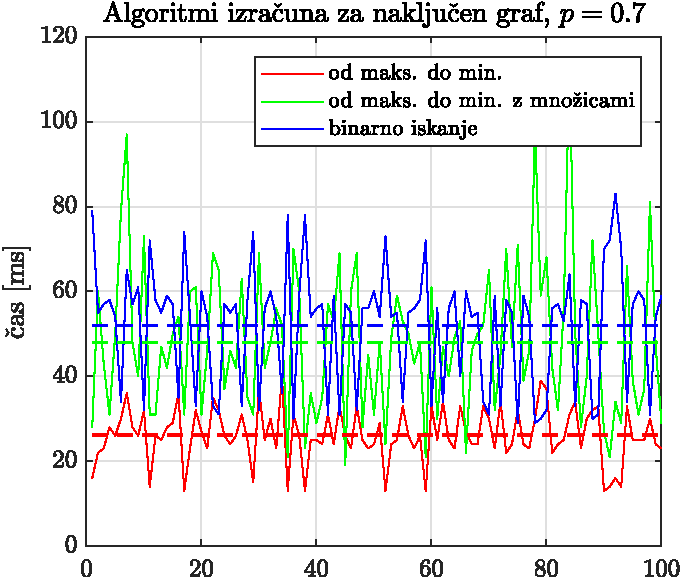
\includegraphics[width=120pt]{../koda/results/plots/zfn_random_15_dense.pdf}
        \caption{Primerjava časov izvajanja treh različic eksponentnega algoritma.}
    \end{figure}
\end{frame}

\begin{frame}{Distribucija ničelne prisile za E-R model}
    \begin{figure}
        \centering
        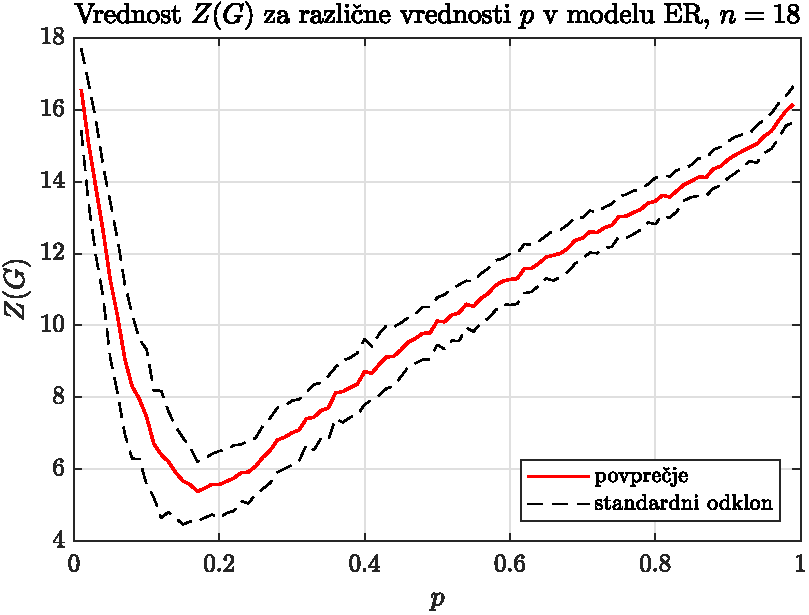
\includegraphics[width=0.49\linewidth]{../koda/results/plots/er_zfn_dist_18_avg.pdf}
        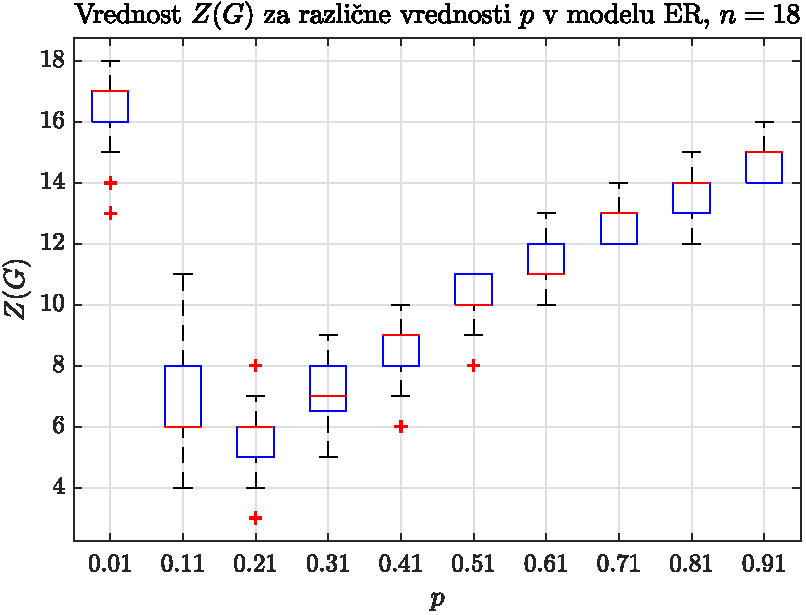
\includegraphics[width=0.49\linewidth]{../koda/results/plots/er_zfn_dist_18_boxplot.pdf}
        \caption{Distribucija ničelne prisile za model Erdős–Rényi, za vsak $p$ je ničelna prisila izračunana za 100 naključno generiranih grafov.}
    \end{figure}
\end{frame}

\begin{frame}{\textsf{NP}-polnost}
    Problem iskanja množice ničelne prisile je $\NP$-težek. 
    
    \bigskip
    
    Problem iskanja povezane množice ničelne prisile je prav tako $\NP$-težek.
    
    \bigskip
    
    Za drevesa znamo ničelno prisilo izračunati v $O(n)$.
\end{frame}

\end{document}
